\documentclass{article}
\usepackage[T1]{fontenc}
\usepackage{polski}
\usepackage{hyperref}
\usepackage{enumerate,xcolor}
\usepackage{graphicx}
\usepackage{titlepic}
\usepackage{listings}
\usepackage{color}

\definecolor{dkgreen}{rgb}{0,0.6,0}
\definecolor{gray}{rgb}{0.5,0.5,0.5}
\definecolor{mauve}{rgb}{0.58,0,0.82}

\lstset{frame=tb,
  language=Java,
  aboveskip=3mm,
  belowskip=3mm,
  showstringspaces=false,
  columns=flexible,
  basicstyle={\small\ttfamily},
  numbers=none,
  numberstyle=\tiny\color{gray},
  keywordstyle=\color{blue},
  commentstyle=\color{dkgreen},
  stringstyle=\color{mauve},
  breaklines=true,
  breakatwhitespace=true,
  tabsize=3
}

\begin{document}
\pagenumbering{arabic}
\title{Podręcznik użytkowania\\
\large{System monitorowania rozproszonych zasobów komputerowych,\\
  np. obciążenia CPU, zużycia pamięci, obciążenia sieci.}}
  \titlepic{
\includegraphics[scale=0.2]{../Znak_graficzny_AGH.png}}

\maketitle
\newpage
\tableofcontents
\newpage
\newcommand{\makered}[1]{\textcolor{red}{#1}}
\newcommand{\makeblue}[1]{\textcolor{blue}{#1}}
\section{Wprowadzenie}
System ma za zadanie monitorowanie rozproszonych zasobów komputerowych. Zainstalowany na komputerze sensor dokonuje pomiarów odpowiednich metryk dla określonych zasobów, zapisuje je w bazie danych, a następnie wysyła dane do monitora.\\\\
Monitor natomiast  zbiera dane od sensorów, a następnie udostępnia pomiary dla klientów. By móc odczytać wszystkie dostępne zasoby i pomiary, odpowiedni serwer webowy czyta dane zawarte w monitorze. Użytkownik korzystający z klienta webowego, może wybrać rodzaj interesującej go metryki.\\\\
\textbf{Architektura systemu:}\\
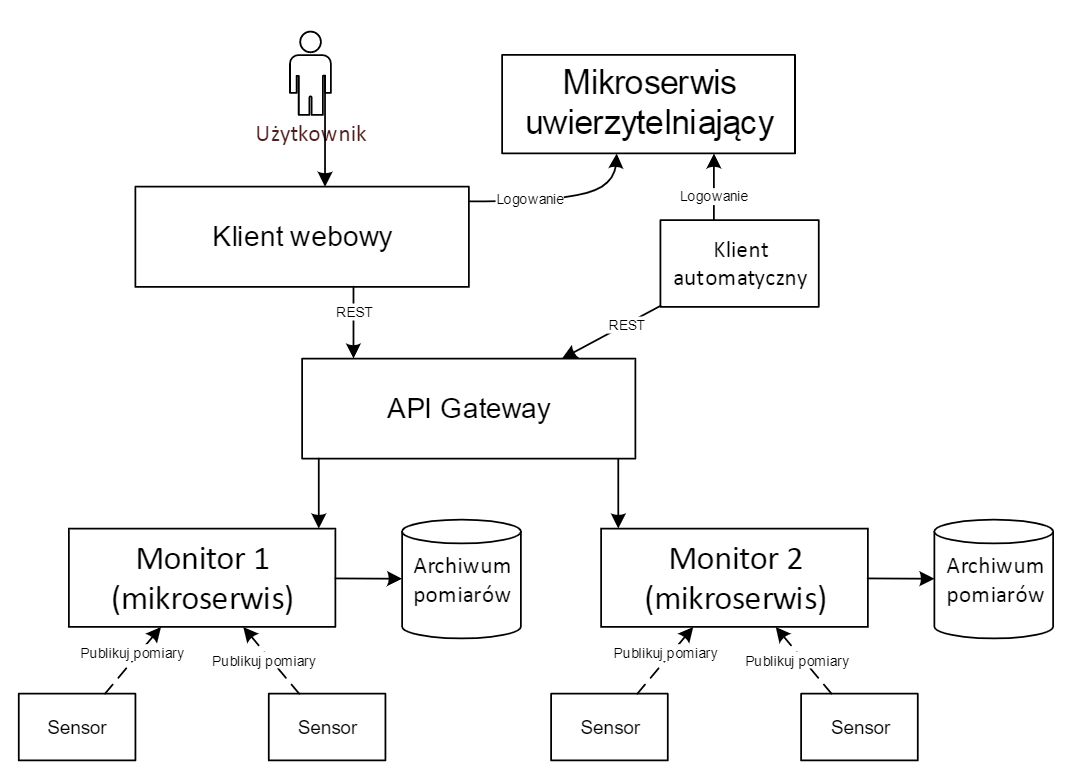
\includegraphics[width=\linewidth]{../ArchitekturaSystemu.png}
\newpage
\section{Monitorowanie zasobów}
Program automatycznie przeszukujący monitorowane zasoby i pomiary w celu wyświetlenia (co pewien czas odświeżonych wyników dla) top 10 najbardziej obciążonych maszyn.

\subsection{Możliwości}
\begin{itemize}
\item Dostęp do API gateway oparty na mikrousłudze uwierzytelniającej.
\item Może podłączyć się do kilku monitorów jednocześnie (za pomocą \texttt{resource/ metrics API Gateway}); przy tym uwzględnia zmiany (wykrywa dodanie nowych lub usunięcie istniejących maszyn z listy monitorowanych zasobów).
\item Wypisuje i co pewien czas (ok. 1 min.) odświeża top 10 najbardziej obciążonych maszyn.
\end{itemize}

\subsection{Opis parametrów}
\begin{lstlisting}
$ ./main.py --help
usage: main.py [-h] -e DATA_ENDPOINT -a AUTH_ENDPOINT -u USERNAME -p PASSWORD               [-d DELAY] [-m METRICS [METRICS ...]]

CLI for monitoring resources.

optional arguments:
  -h, --help            show this help message and exit
  -e DATA_ENDPOINT, --data-endpoint DATA_ENDPOINT
                        Enpoint for gathering monitoring data.
  -a AUTH_ENDPOINT, --auth-endpoint AUTH_ENDPOINT
                        Enpoint for authentication microservice.
  -u USERNAME, --username USERNAME
                        Username for API Gateway authentication.
  -p PASSWORD, --password PASSWORD
                        Password for API Gateway authentication.
  -d DELAY, --delay DELAY
                        Delay time (default 2 sec).
  -m METRICS [METRICS ...], --metrics METRICS [METRICS ...]
                        Metrics to show - space separated list. First element
                        defines key for sorting to display top resources
                        (default cpu).
\end{lstlisting}

Dodatkowo warto pamiętać, że:

\begin{itemize}
\item \texttt{DELAY} - jest parametrem periodycznego odświeżania dashboadu (tabeli), natomiast pobieranie dzieje się w osobnej korutynie w pętli.
\item \texttt{METRICS} - pierwsza metryka w liście jest parametrem sortowania "top"
\item \texttt{USERNAME}, \texttt{PASSWORD} - stanowią dane użytkownika
\end{itemize}

\section{Użytkowanie systemu}
System webowy znajduje się pod adresem:\\\\
\centerline{\url{http://web-client-pz.azurewebsites.net/}}\\\\
Po uruchomieniu lokalnie systemu, klient webowy znajduje się pod adresem:\\\\
\centerline{\url{http://localhost:4200}}\\\\

\subsection{Logowanie}
Po wejściu na stronę należy zalogować się do systemu. Aby tego dokonać w pola należy wpisać:
\begin{itemize}
\item login: \texttt{enduser}, password: \texttt{password}
\item login: \texttt{enduser2}, password: \texttt{password2}
\end{itemize}
Po zalogowaniu się do systemu, wyświetlane są ostatnie pomiary metryk z różnych zasobów tj:
\begin{itemize}
\item obciążenie CPU
\item zużycie pamięci
\end{itemize}
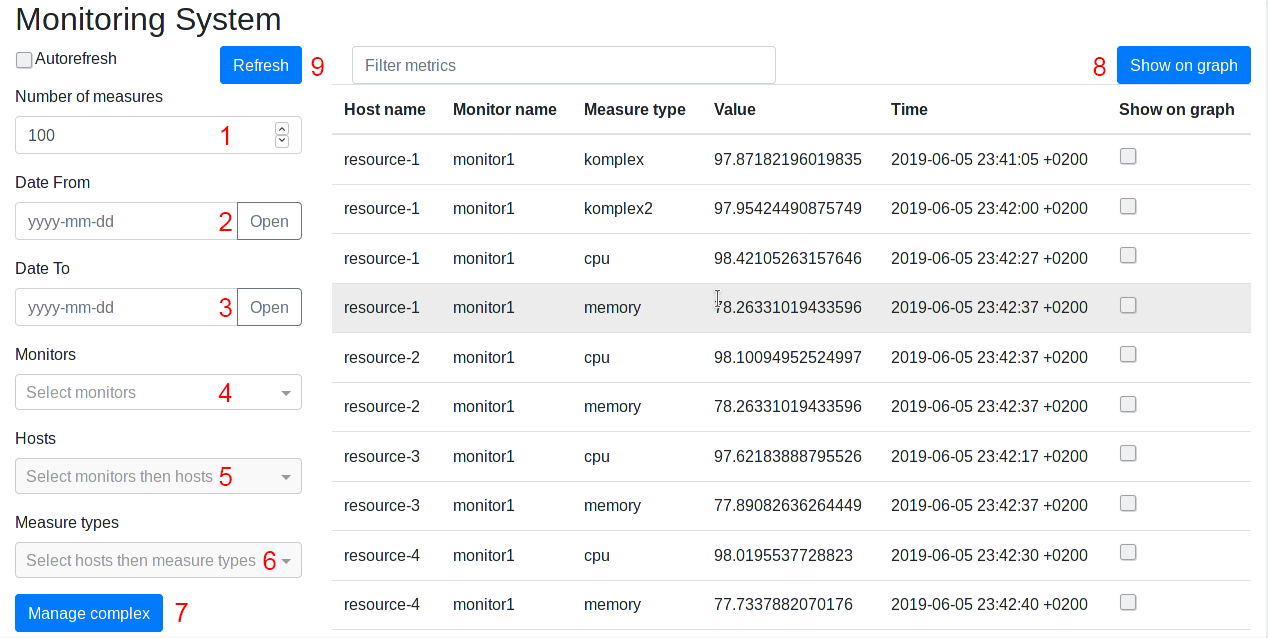
\includegraphics[width=\linewidth]{../screen/ResourceMonitor.png}

\newpage
\subsection{Zarządzanie metrykami}
Ilość metryk do wyświetlenia, jest domyślnie ustawiona na 100. Po lewej stronie w polu \textbf{Number of measures} \makered{(1)} istnieje możliwość zmiany tej wartości. Użytkownik posiada także możliwość wskazania zakresu czasu kiedy zostały dokonane pomiary metryk - sekcja \textbf{Date From} i \textbf{Date To} \makered{(2-3)} \\\\ 
Użytkownik może także wskazać, aby na liście pomiarów pokazały się tylko:
\begin{itemize}
\item \textbf{Monitors} - Odczytane metryki z danego monitora \makered{(4)}
\item \textbf{Hosts} - Odczytane metryki z danego hosta \makered{(5)}
\item \textbf{Measure types} - Odczytane konkretne metryki \makered{(6)}
\end{itemize}
Aby zatwierdzić należy wcisnąć \makeblue{Refresh} \makered{(9)}.\\\\ 
Przykładowa wyświetlona lista pomiarów po filtracji:\\\\
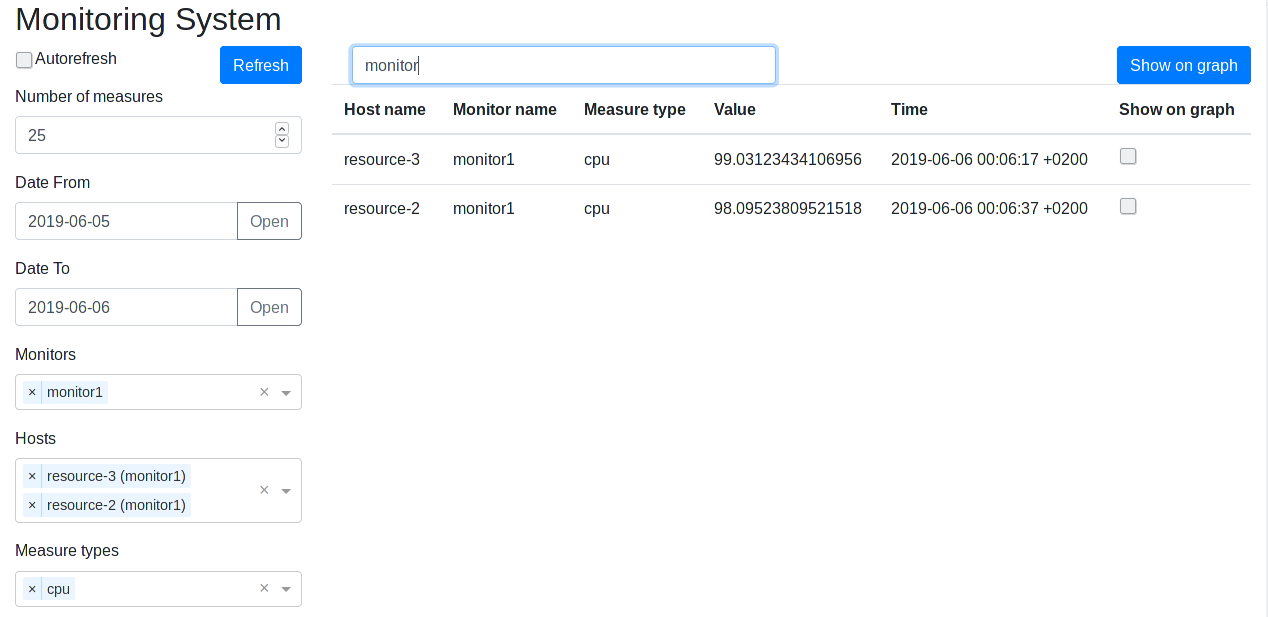
\includegraphics[width=\linewidth]{../screen/ResourceMonitorFilter.png}

\newpage
\subsection{Wykresy}
Po dokonaniu filtracji użytkownik może wyświetlić dane w postaci wykresu. Po prawej stronie, przy każdej metryce, znajduje się znacznik, który należy kliknąć, jeśli chcemy aby dane tej metryki pojawiły się na wykresie. Klikając w \makeblue{Show on graph} znajdujący się w prawym górnym rogu. \makered{(8)} na stronie pojawia się wykres.
\begin{figure}[h]
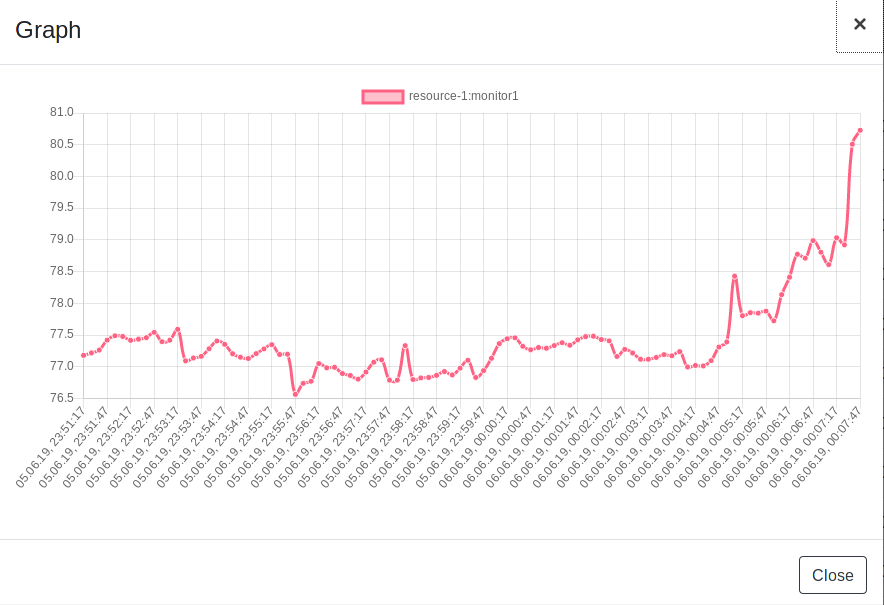
\includegraphics[scale=0.35]{../screen/Wykres.png}
\centering
\caption{Wykres obciążenia CPU jednego hosta}
\end{figure}
\begin{figure}[h]
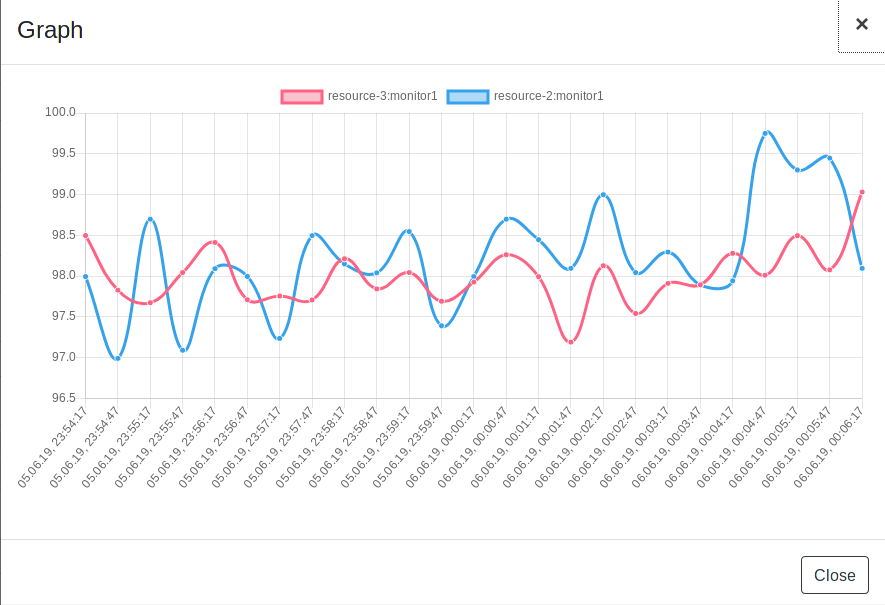
\includegraphics[scale=0.35]{../screen/Wykres2.png}
\centering
\caption{Wykres obciążenia CPU dwóch hostów}
\end{figure}

\newpage
\subsection{Zasoby złożone}

Użytkownik posiada także możliwość tworzenia oraz usuwania pomiarów złożonych. Pomiar ten jest średnią ruchomą danej metryki. Aby tego dokonać, lewym dolnym rogu należy wcisnąć przycisk \makeblue{Manage complex} \makered{(7)}\\\\
Na ekranie po prawej stronie, powinna się pojawić lista obecnych pomiarów złożonych. Po lewej zaś, można utworzyć nowy pomiar.\\
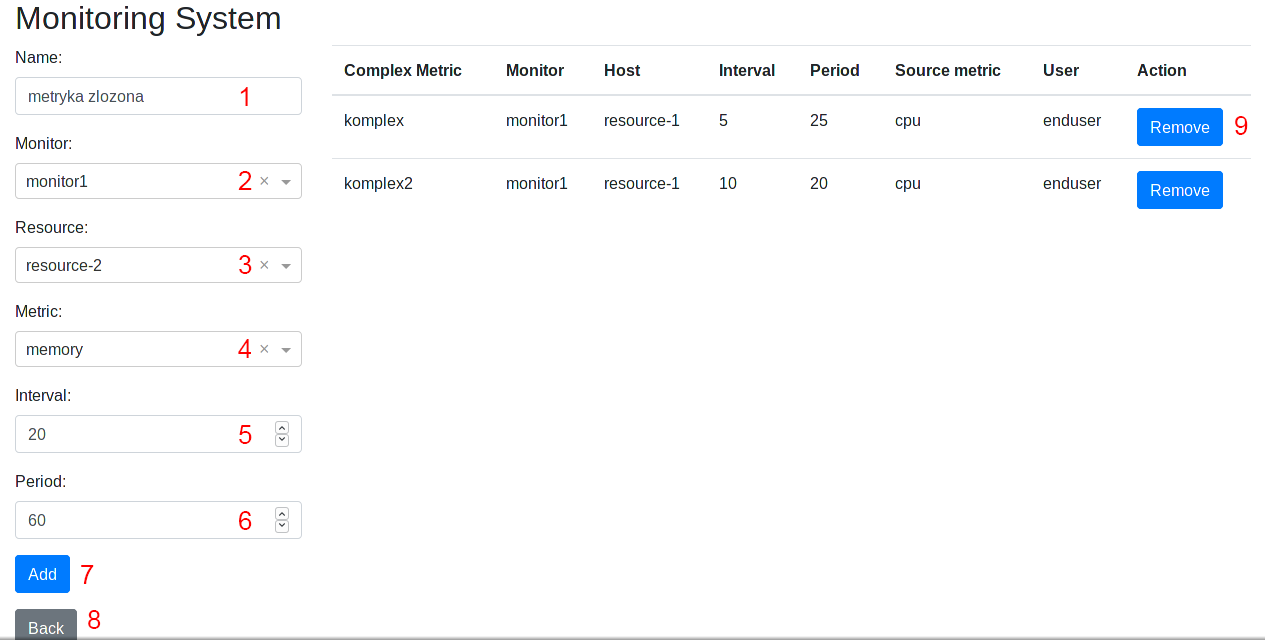
\includegraphics[width=\linewidth]{../screen/ComplexSystem2.png}
 Aby tego dokonać w odpowiednich polach należy wpisać.\\
\begin{enumerate}[\begingroup\color{red} (1)\endgroup]
\item - \textbf{Name} - Nazwę pomiaru
\item - \textbf{Monitor} - Z jakiego monitora mają być dokonywane pomiary
\item - \textbf{Resource} - Z jakiego zasobu  
\item - \textbf{Metric} - Jaka jest to metryka
\item - \textbf{Interval} - Długość okna czasowego - w min. - (np. średnia z 20 minut)
\item - \textbf{Period} - Częstotliwość obliczania - w min.
\end{enumerate}
W celu zatwierdzenia należy wcisnąć \makeblue{Add} \makered{(7)}.\\\\ 
Jeżeli użytkownik zdecyduje się usunąć dany pomiar złożony po prawej stronie znajduje się przycisk \makeblue{Remove} \makered{(9)}, który należy kliknąć. Jeżeli użytkownik chce powrócić do listy pomiarów metryk, należy kliknąć przycisk \makeblue{Back} \makered{(8)}, znajdujący się po prawej dolnej stronie.

\end{document}
